We use a Bayesian approach to model comparison to find out which model
best explains the data described in the previous section
\cite{VandekerckhoveMatzke2013:Model-Compariso}. The models under
investigation have unspecified parameters: the speaker's degree of of
rationality $\lambda_\mathrm{S}$, the cost of adjectives $c$, and, for
those listener models that have an action-oriented communication goal
, the listener's degree of rationality $\lambda_\mathrm{L}$. Since
there is no principled theory to determine the value of the
parameters, we will rely on relatively uninformed hyperpriors
(so-called to distinguish them from the salience priors). Based on a
specification of hyperpriors, we calculate the models' \emph{evidence}
and compare them by their \emph{Bayes factors}. The evidence of a
model $M$ is the weighted average of the likelihood of observing the
data under all parameter values:
\begin{align}
  \label{BMA}
  \mathrm{Ev}(M)= \int \Pr(\theta) \cdot p(D | M, \theta)\, \mathrm{d}\theta,
\end{align}
where $\Pr(\theta)$ is the hyperprior over parameter(-tuple) $\theta$
associated with $M$ and $D$ is the observed data. The Bayes factor
$K^{M_1}_{M_2}$ is a comparative measure for the plausibility of model
$M_1$ over $M_2$, given their respective hyperpriors and the data in
question:
\begin{align}
  K^{M_1}_{M_2} = \frac{\mathrm{Ev}(M_1)}{\mathrm{Ev}(M_2)} \enspace .
\end{align}
Model $M_1$ makes the data more likely whenever $K^{M_1}_{M_2}$, but
normally only a Bayes factor $K^{M_1}_{M_2} >3$ (or sometimes
$K^{M_1}_{M_2} > 5$) is considered substantial. Values $K^{M_1}_{M_2}
> 10$ are considered strong evidence.

In a sense, comparison by Bayes factors is comparing models in a wider
sense of the term: we actually compare pairs consisting of a model and
its associated hyperprior. For clarity, we refer henceforth to a
model-hyperprior pair as a Model.

\paragraph{Speaker data.} First we look at the speaker models $\sigma_{xy},\
x\in\{a,b\},y\in\{\mathcal{U},\mathcal{S}\}$. Each model has two
parameters $\lambda_\mathrm{S}$ and $c$. We assume that they are
independent of each other:
\begin{equation}\label{hyper-speaker-independent}
\Pr(\lambda_\mathrm{S},c)=\Pr(\lambda_\mathrm{S}) \cdot \Pr(c) \enspace .
\end{equation}
We are uncertain about the rationality of the speaker:
\begin{equation}\label{hyper-speaker-lambda}
\Pr(\lambda_\mathrm{S})= \mathcal{U}_{(0,11)}(\lambda_\mathrm{S}),
\end{equation}
which is a uniform distribution over $(0,11)$. Excluding
$\lambda$-values $\ge 11$ serves practical purposes only, but is
innocuous since the regions of maximum a posteriori likelihood of
$\lambda$ lies safely in the chosen interval for all models. Next, to
allow for the possibility of speaker preferences (nouns over
adjectives or vice versa), we consider two types of hyperpriors for
costs $c$. The first hyperprior has $\Pr(c)= \delta(c)$, the Dirac
delta distribution, that assigns all probability mass $1$ to
$c=0$. This captures the assumption that there is no speaker
preference. The second hyperprior is $\mathcal{U}_{(-0.4,0.4)}$, which
captures the notion that a preference exists, without commitment to
either direction. We restrict our attention to the interval
$(-0.4,0.4)$, because we consider higher levels of cost implausible,
given that utilities for successful communication live in $[0,1]$ and
that we believe that strive for communicative success should outrank
preference satisfaction in a rational model of communication. Taken
together, there are four speaker models, two hyperpriors for each, so
that we compare eight Models with respect to their evidences.

Evidences of speaker Models were calculated by grid approximation. The
results are shown in Table \ref{table:speaker mod}. We can see
\todo{include Hinton diagrams?} that the data very strongly supports
speaker models that do not take the listener's perceptual salience
into account. Also, it seems that action-oriented models are slightly
better than their belief-oriented counterparts, even though the
relevant Bayes factors are not substantial by common
standards. Finally, our data makes each speaker Model that does allow
for a speaker preference strongly more plausible than its
counterpart that does not. A look at the posterior likelihood of $c$
for each speaker model informs us that our data supports the belief
that the speakers have a preference for nouns, see
Figure~\ref{fig:cost_post_s}. \todo{improve plot}
%
\begin{table}[htb] 
  \centering 
  \caption{Evidences of speaker Models}
  \begin{tabular}{lcccc}
    support of $P(c)$ 
    & $\sigma_{\mathrm{b}\mathcal{U}}$
    & $\sigma_{\mathrm{a}\mathcal{U}}$
    & $\sigma_{\mathrm{b}\mathcal{S}}$
    & $\sigma_{\mathrm{a}\mathcal{S}}$
    \\ \midrule
    $[0,0]$
    & 4.93e-30
    & 3.56e-30
    & 5.92e-46
    & 3.09e-69
    \\
    $(-0.4,0.4)$
    & 5.04e-15
    & 4.02e-15
    & 4.28e-36
    & 3.27e-61
  \end{tabular} 
  \label{table:speaker mod}
\end{table}
%
\begin{figure}[htb]
  \centering
  \caption{Posterior distributions over costs given the data for each
    speaker model.}
  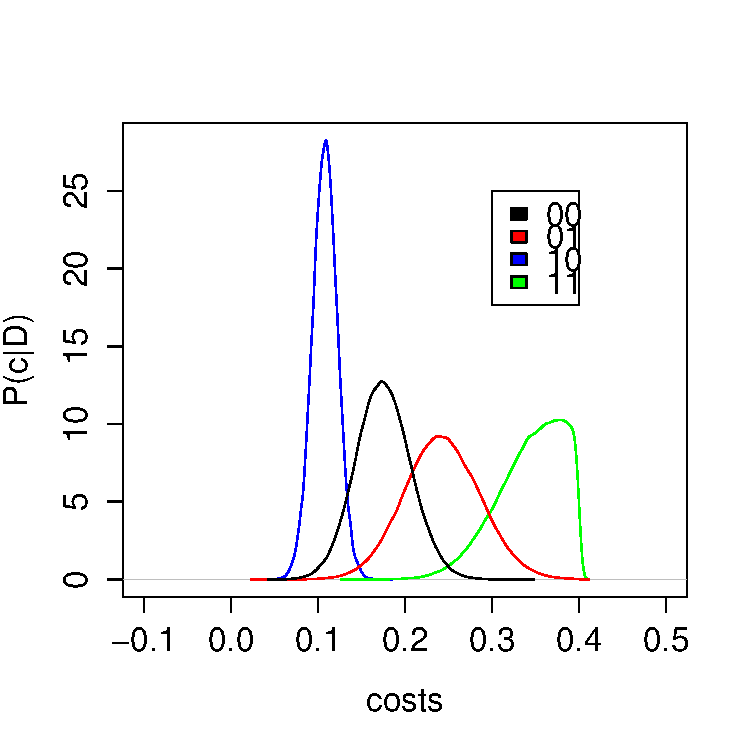
\includegraphics[width=0.5\textwidth]{pics/cost_post_s.pdf}
  \label{fig:cost_post_s}
\end{figure}
%
In sum, our data supports the belief that the speaker does not take
into account the preceptual salience of the listener, while having her
own preference for shape terms over color terms.


\paragraph{Listener data.} Each listener models has a speaker model
nested inside as a belief of the listener about the speaker's
behavior. Section~XYZ \todo{cross-reference} introduced a total of 16
potentially relevant listener models, but we will focus on a selection
only. For one, we restrict our attention to those listener models that
are either entirely belief-based or entirely action-based. In other
words, we exclude models like
$\rho_{\mathrm{a}\cdot}(\sigma_{\mathrm{b}\cdot})$ where the receiver
part assumes an action-based goal structure and the speaker part a
belief-based goal structure. For another, we assume that the
listener's model of the speaker is a reasonable one and therefore put
to the side listener models that have speaker models that are highly
implausible, given the speaker data as discussed above. Effectively,
this discards listener models that include a speaker models that take
the listener's salience prior into account. These two principled
restrictions leave us with four listener models to compare.

Further variation comes from different relevant
hyperpriors. Belief-based models of the listener have the same
parameters as speaker models: the speaker's rationality
$\lambda_\mathrm{S}$ and the speaker's preference costs
$c$. Importantly though, hyperpriors over $\lambda_\mathrm{S}$ and
$c$, although formally parallel to those for speaker models, have a
different interpretation in listener models where they capture our
prior beliefs about the listeners' beliefs about the speakers' likely
rationality and preferences. This is true as well for action-based
models, which also have an additional parameter
$\lambda_\mathrm{L}$. Hyperpriors for the latter encode our prior
beliefs about the listener's actual rationality.

We consider a variety of hyperpriors that differ with respect to
whether they take the speaker's costs into account, whether the
listener's beliefs about the speaker's rationality and preferences are
uninformed (i.e., flat) or informed (i.e., given by the posterior
likelihood of parameters given the actual speaker data) and, in
action-based models, whether the listener's level of rationality
corresponds to his ``informed'' beliefs. The latter option effectively
implements the assumption that there is a tight correlation between
the speaker's actual rationality, the listener's actual rationality
and the listener's beliefs about the speaker's rationality.

Concretely, we call ``flat w/o costs'' the hyperpriors:
\begin{align*}
  \Pr(\lambda_\mathrm{S},c) & =
  \mathcal{U}_{(0,11)}(\lambda_\mathrm{S}) \cdot
  \delta(c) \\
  \Pr(\lambda_\mathrm{S},c,\lambda_\mathrm{L}) & = 
  \mathcal{U}_{(0,11)}(\lambda_\mathrm{S}) \cdot
    \delta(c) \cdot  \mathcal{U}_{(0,11)}(
    \lambda_\mathrm{L}),
\end{align*}
for belief-based and action-based models respectively. Hyperpriors
``flat with costs'' take a wider range of speaker preferences into
account: 
\begin{align*}
  \Pr(\lambda_\mathrm{S},c) & =
  \mathcal{U}_{(0,11)}(\lambda_\mathrm{S}) \cdot
  \mathcal{U}_{(-0.4,0.4)}(c) \\
  \Pr(\lambda_\mathrm{S},c,\lambda_\mathrm{L}) & = 
  \mathcal{U}_{(0,11)}(\lambda_\mathrm{S}) \cdot
    \mathcal{U}_{(-0.4,0.4)}(c) \cdot  \mathcal{U}_{(0,11)}(
    \lambda_\mathrm{L}) \enspace .
\end{align*}

Hyperpriors that capture the idea that the listener's beliefs are good
guesses of speaker behavior are modeled as if informed by the data
from the speaker experiments:
\begin{align*}
  \Pr(\lambda_\mathrm{S},c) & = \Pr(\lambda_\mathrm{S},c \mid D_\mathrm{S}, M_\mathrm{S}) \\
  \Pr(\lambda_\mathrm{S},c,\lambda_\mathrm{L}) & = 
   \Pr(\lambda_\mathrm{S},c \mid D_\mathrm{S}, M_\mathrm{S}) \cdot  \mathcal{U}_{(0,11)}(
    \lambda_\mathrm{L}) \enspace .
\end{align*}
Here, $D_\mathrm{S}$ is the data from the speaker experiments, and
$M_\mathrm{S}$ the relevant speaker model. For a given listener model,
we consider only the embedded speaker model as relevant. We call
hyperpriors of the above form ``informed'' or, in the case of
action-based models, ``informed uncorrelated''. We distinguish the
latter from ``informed correlated'' hyperpriors of the form:
\begin{align*}
  \Pr(\lambda_\mathrm{S},c,\lambda_\mathrm{L}) & = 
   \Pr(\lambda_\mathrm{S},c \mid D_\mathrm{S}, M_\mathrm{S}) \cdot \Pr(\lambda_\mathrm{L} \mid D_\mathrm{S}, M_\mathrm{S}),
\end{align*}
where the listener's rationality parameter is distributed according to
the relevant posterior (marginalized over costs). All of the three
types of informed hyperpriors were tested in two varieties: whether
the listener takes the sender's preferences into account or not. If he
does not, the posterior $\Pr(\lambda_\mathrm{S},c \mid D_\mathrm{S},
M_\mathrm{S})$ is derived from a speaker-hyperprior $\Pr(c) =
\delta{c}$; otherwise from $\Pr(c) = \mathcal{U}_{(-0.4,0.4)}(c)$.

Taken together, we consider two belief-based models, paired with four
hyperpriors, and two action-based models, paired with six hyperpriors
(see Table~XYZ\todo{reference}). Comparing these ten Models is meant
to address the following general questions:
\begin{enumerate}
\item Is the goal structure assumed by participants in our task
  belief-based or action-based?
\item Does the listener take the estimated salience prior into account
  or not?
\item Is the listener's belief in the speaker's level of rationality
  ``correct'', i.e., in line with the observed speaker data?
\item Is the listener's level of rationality related to the speaker's
  actual level of rationality?
\end{enumerate}




\begin{table}[htb]
  \centering
  \caption{asdf}
  \begin{tabular}{llr}
    belief-based 
    & action-based
    & 
    \\
    $\Pr(\lambda_\mathrm{S},c)$
    & $\Pr(\lambda_\mathrm{S},c,\lambda_\mathrm{L})$
    & label
    \\ \midrule
    $\mathcal{U}_{(0,11)}(\lambda_\mathrm{S}) \cdot \mathcal{U}_{[0,0]}(c)$
    & $\mathcal{U}_{(0,11)}(\lambda_\mathrm{S}) \cdot
    \mathcal{U}_{[0,0]}(c) \cdot  \mathcal{U}_{(0,11)}(
    \lambda_\mathrm{L})$
    & flat, w/o costs
    \\
    $\mathcal{U}_{(0,11)}(\lambda_\mathrm{S}) \cdot \mathcal{U}_{(-0.4,0.4)}(c)$
    & $\mathcal{U}_{(0,11)}(\lambda_\mathrm{S}) \cdot
    \mathcal{U}_{(-0.4,0.4)}(c) \cdot  \mathcal{U}_{(0,11)}(
    \lambda_\mathrm{L})$
    & flat, with costs
    \\
    $\Pr(\lambda_\mathrm{S},c \mid D_\mathrm{S}, M_\mathrm{S})$
    & $\Pr(\lambda_\mathrm{S},c \mid D_\mathrm{S}, M_\mathrm{S}) \cdot  \mathcal{U}_{(0,11)}(
    \lambda_\mathrm{L})$
    & informed uncorrelated, w/o costs
    \\
    $\mathcal{U}_{(0,11)}(\lambda_\mathrm{S}) \cdot \mathcal{U}_{(-0.4,0.4)}(c)$
    & $\mathcal{U}_{(0,11)}(\lambda_\mathrm{S}) \cdot
    \mathcal{U}_{(-0.4,0.4)}(c) \cdot  \mathcal{U}_{(0,11)}(
    \lambda_\mathrm{L})$
    & informed uncorrelated, with costs
    \\
  \end{tabular}
  \label{tab:hyperpriors_l}
\end{table}


\vspace{1cm}
\hrule
\vspace{1cm}



 Since we want to know how such a belief correlates with the
actual production, we put two kinds of hyperpriors under
investigation. On the one hand, the flat-independent hyperpriors treat
different parameters as independent:
\begin{equation}\label{hyper-listener-independent}
\Pr(\lambda_\mathrm{S},c,\lambda_\mathrm{L})=\mathcal{U}_{(0,11)}(\lambda_\mathrm{S}) \cdot \Pr(c) \cdot  \mathcal{U}_{(0,11)}( \lambda_\mathrm{L}) \enspace .
\end{equation}
On the other hand, the true-correlated hyperpriors use the data from the speaker condition to estimate the hyperpriors for $\lambda_\mathrm{S}$ and $c$, and let $\lambda_\mathrm{L}$ have the same distribution as $\lambda_\mathrm{S}$:
\begin{equation}\label{hyper-listener-independent}
\Pr(\lambda_\mathrm{S},c,\lambda_\mathrm{L})=\mathcal{U}_{(0,11)}(\lambda_\mathrm{S} \mid D_\mathrm{S}, M_\mathrm{S}) \,\Pr(c\mid D_\mathrm{S}, M_\mathrm{S})  \,\mathcal{U}_{(0,11)}( \lambda_\mathrm{L} \mid D_\mathrm{S}, M_\mathrm{S}),
\end{equation}
and thus put a stronger constraint on the listener's belief about the speaker. 

The comparison result of the speaker models are shown in Table \ref{table:listener mod}. The best model, which is substantially better than the rest, is action-oriented and takes perceptual salience into account. It has a true-correlated speaker model which is action-oriented and does not take perceptual salience nor speaker preference into account. Note that the nested speaker model is different from the best actual speaker model only in that it does not incorporate speaker preference.  

\begin{table}[htb] 
\caption{Listener Model Comparison}
  \centering 
  \begin{tabular}{ccccc}
    rank
    & model
    & hyperprior
    & sp.~pref.
    & evidence 
    \\ \hline
    1 
    & $\rho_{\mathrm{a}\mathcal{S}}(\sigma_{\mathrm{a}\mathcal{U}})$
    & true correlated
    & $-$
    & 1.11E-003
    \\ \\
    2 
    & $\rho_{\mathrm{ a}\mathcal{S}}(\sigma_{\mathrm{b}\mathcal{U}})$
    & true correlated
    & $-$
    & 2.36E-004
    \\     
    3 
    & $\rho_{\mathrm{b}\mathcal{U}}(\sigma_{\mathrm{b}\mathcal{S}})$
    & flat independent \quad
    & adj.~or nouns \quad
    & 1.29E-004
    \\     
    4 
    & $\rho_{\mathrm{a}\mathcal{U}}(\sigma_{\mathrm{b}\mathcal{S}})$
    & flat independent
    & none
    & 9.94E-005
    \\     
    5 
    & $\rho_{\mathrm{a}\mathcal{U}}(\sigma_{\mathrm{b}\mathcal{S}})$
    & flat independent
    & adj.~or nouns
    & 8.79E-005
    \\
    $\vdots$\\
    14 
    & $\rho_{\mathrm{b}\mathcal{S}}(\sigma_{\mathrm{b}\mathcal{U}})$
    & flat independent
    & adj.~or nouns
    & 5.31E-005
    \\
    $\vdots$\\
    19 
    & $\rho_{\mathrm{b}\mathcal{S}}(\sigma_{\mathrm{b}\mathcal{U}})$
    & true correlated
    & $-$
    & 2.91E-005
    \\
    $\vdots$
  \end{tabular}
  \label{table:listener mod}
\end{table}

Combining the model comparison results for both the speaker and the listener models, it seems that if we treat the speaker's preference as some lexical salience which together with the listener's perceptual salience constitutes the contextual salience of the referential game, then contextual salience actually manifests \emph{lack of} common knowledge between the speaker and the listener rather than the presence of it, since they both have some preference that biases their decisions but they are unaware of each other's such preference. However, there is indeed something common between the speaker and the listener, i.e. the distribution of the degree of rationality. Also, the listener's belief about the speaker is correct modulo the speaker's private lexical salience. 


%%% Local Variables: 
%%% mode: latex
%%% TeX-master: "main"
%%% TeX-PDF-mode: t
%%% End: